\chapter{CORDIC}
\section{Algoritmo de CORDIC}
\todo{Revisar de nuevo si las formulas estan correctas. Comentar Linear/Circular/Hyperbolic}

En esta sección se describirá el funcionamiento principal del algoritmo CORDIC según descrito por Jack E. Volder.

La rotación de un vector de dos dimensiones $\boldsymbol{p_{0}} = [x_{0},y_{0}]$ con un ángulo $\theta$ para obtener un vector $\boldsymbol{p_{n}} = [x_{n},y_{n}]$ se puede realizar con un producto matriz $\boldsymbol{p_{n}}$ = $\boldsymbol{R_{p_{0}}}$, donde $\textbf{R}$ es la matriz de rotación.

\[ \textbf{R} = \begin{bmatrix}
\cos{\theta} & -\sin{\theta} 	\\[0.3em]
\sin{\theta}  & \cos{\theta} 			\\[0.3em]
\end{bmatrix} \]

Si sacamos el coseno de la matriz de rotación, se puede obtener un valor K, el cual se convierte en una constante.

\[ \textbf{R} = [(1 + \tan^2{\theta})^{\sfrac{-1}{2}}] \begin{bmatrix}
1 & -\tan{\theta} 	\\[0.3em]
\tan{\theta}  & 1 			\\[0.3em]
\end{bmatrix} \]

Nombraremos como $K = [(1 + \tan^2{\theta})^{\sfrac{-1}{2}}]$ el factor escala. Eliminando $K$ obtenemos una matriz de pseudo-rotación $\boldsymbol{R_{c}}$ tal que

\[ \boldsymbol{R_{c}} = \begin{bmatrix}
1 & -\tan{\theta} 	\\[0.3em]
\tan{\theta}  & 1 			\\[0.3em]
\end{bmatrix} \]

La operación pseudo-rotación realizada sobre el vector $p_{0}$ por un ángulo $\theta$ y cambia su magnitud por un factor $K = \cos{\theta}$.

Para obtener la simplicidad dentro del hardware necesitamos:

\begin{itemize}
	\item Descomponer las rotaciones en una secuencia de rotaciones elementales con ángulos predefinidos que se pueda implementar con un coste hardware mínimo.
	\item Eliminar el factor escala $K$, ya sea finalizando la operación con una simple multiplicación o ignorarlo directamente.
\end{itemize}

En primer lugar, CORDIC realiza una rotación iterativa con una lista de ángulos predefinidos $\alpha_{i} = \arctan({2^{-i}})$ de manera que $\tan({\alpha_{i}}) = 2^{-i}$ se puede implementar en hardware como un desplazamiento de $i$ posiciones.

Ya que estamos limitando la operación $\tan{\theta}$ a una lista de rangos predefinidos anteriormente podemos asumir que

\[
	K_{i} = \frac{1}{sqrt{(1+2^{-2_{i}})}}
\]

El factor escala $K_{i}$ altera la magnitud del vector a rotar independientemente del valor del ángulo. 

Ya que el factor escala no depende del ángulo de las micro-rotaciones, no necesitamos incluir el factor dentro de las operaciones, lo que nos da $\boldmath{p_{n} = R_{c}p_{0}}$.

El factor final $K$ tiene un valor de $~1.6467605$, por lo cual simplemente se puede escalar el valor final por $K$.

Los valores finales que nos interesan son los siguientes:

\[
\begin{matrix}
	x_{i+1} = x_{i} - \delta_{i} \times 2^{-i} \times y_{i} \\
	y_{i+1} = y_{i} - \delta_{i} \times 2^{-i} \times x_{i} \\
	\omega_{i+1} =  \omega_{i} - \delta_{i} \times \alpha_{i}
\end{matrix}
\]

\todo[inline]{arreglar las figuras. Tal vez se arreglen solas.}
\begin{figure}[ht]
	\centering
	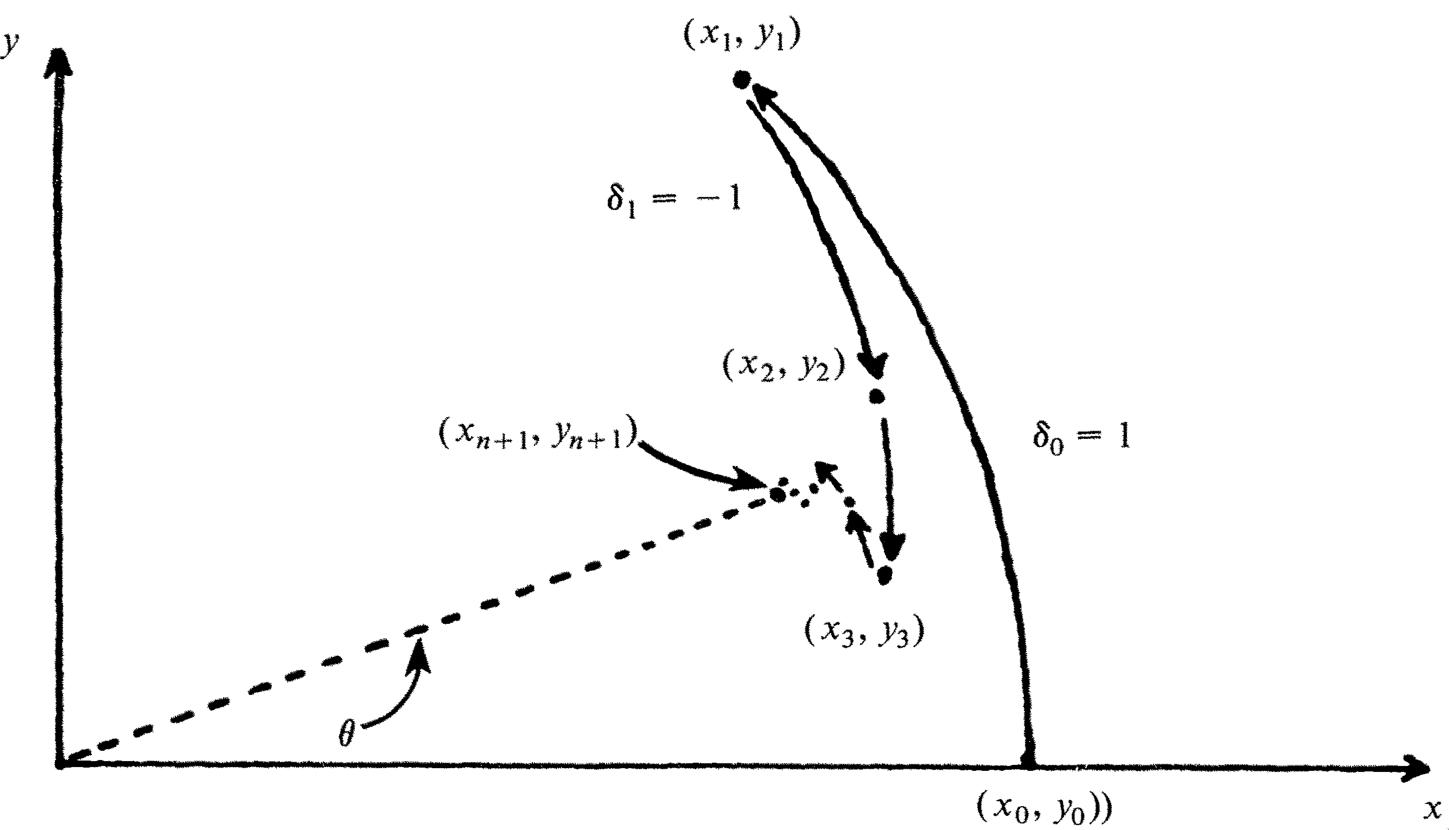
\includegraphics[width=\textwidth]{archivos/CORDIC/RotationMode.png}
	\caption{Rotation Mode}
	\label{graf:RM}
\end{figure}

\begin{figure}[ht]
	\centering
	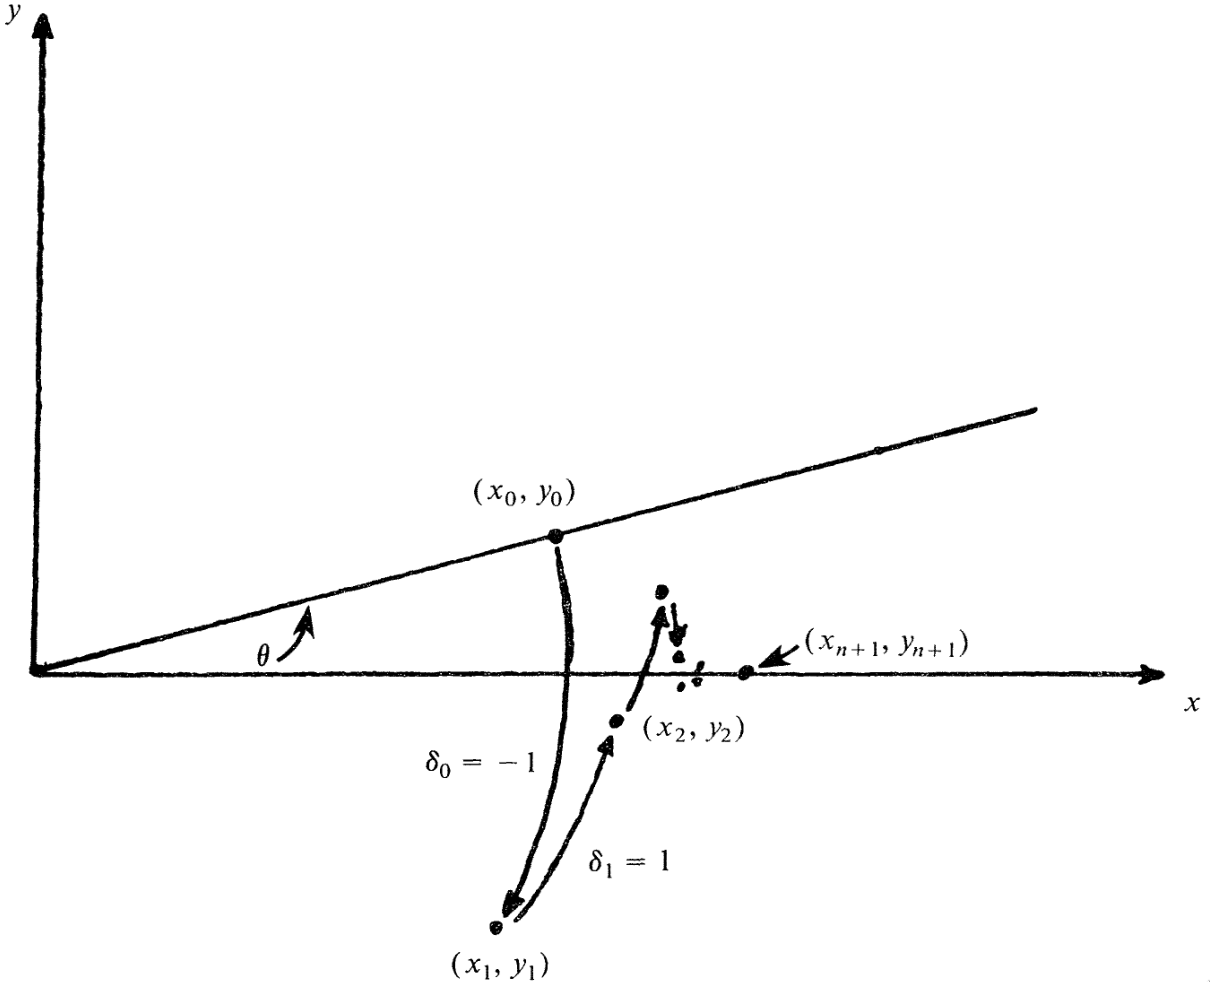
\includegraphics[width=\textwidth]{archivos/CORDIC/VectoringMode.png}
	\caption{Vectoring Mode}
	\label{graf:VM}
\end{figure}

CORDIC puede operar de dos formas: \textit{Rotation Mode} (RM) (\ref{graf:RM}) y \textit{Vectoring Mode} (VM) (\ref{graf:VM}). La principal diferencia es en como se eligen las micro-rotaciones. En RM, la dirección de cada micro-rotación depende del signo de $\omega_{i}$. Si $\omega_{i}$ es positivo $\delta_{i} = 1$, si no $\delta_{i} = -1$. En VM, el vector se rota hacia el eje de $x$, por lo que la componente $y$ tiende a 0.

Posteriormente, J.S. Walther propuso un CORDIC generalizado unificado para realizar multitud de operaciones matemáticas, pero esto se encuentra fuera del alcance de esta memoria.

\section{Mejoras a CORDIC}

En el apartado de introducción se explicaron algunas aplicaciones de CORDIC, sin tener detallar el tipo o las modificaciones realizadas. En este apartado se muestran algunas de estas mejoras.



\chapter{CORDIC y punto flotante}
\todo{Que hacer con las figuras. section o chapter?}

\cite{parker_abstract_2011} Muestra claramente algunos de los problemas que conlleva implementar el estándar del IEEE 754 en hardware. En concreto estos problemas son relaciones con algunos aspectos de las FPGAs, pero puede ser aplicable a cualquier problema donde el hardware es limitado. Algunos de estos problemas son:

\begin{itemize}
	\item La representación de la mantisa incluye un 1 implícito. El valor real va desde [1:1.999..] en vez de [0:0.000..]. 
	\item En vez de usar complemento a dos, el estándar incluye un bit de signo.
	\item Cada operación aritmética conlleva una normalización de la mantisa para alinear el punto decimal hacia la izquierda, además de tener que ajustar el exponente de forma acorde.
	\item VHDL y Verilog no tienen una implementación de operaciones con punto flotante. Un lenguaje de descripción de hardware mas nuevo, como SystemVerilog si tiene estas operaciones, pero la complejidad de ellas conlleva a perder mucho espacio, el cual puede estar bastante limitado en las FPGAs.
\end{itemize}

Dentro de la evolución del uso de punto flotante en el método hay una variedad importante de arquitecturas y algoritmos de CORDIC.

Una de las primeras implementaciones de un tipo de punto flotante, explicado por \cite{leibson_9100_2005} fue sobre el año 1954 con la calculadora de sobremesa HP 9100A. La calculadora tenía 16 registros, numerados de forma hexadecimal y podía guardar valores de punto flotante con 10 dígitos de mantisa y 2 dígitos de exponente en formato BCD. La mantisa y el exponente podían guardar valores positivos y negativos.

Según \cite{walther_unified_1971}, la primera implementación de punto flotante tenía grandes limitaciones en el tema de hardware a la hora de convertir los valores entre BCD a base 2 y, además, no había un estándar de punto flotante en aquel entonces, por lo que cada diseñador creaba su propio formato.

\todo{Look at 1993 and check if they followed up with what the stated in the conclusion}
\begin{figure}[ht]
	\centering
	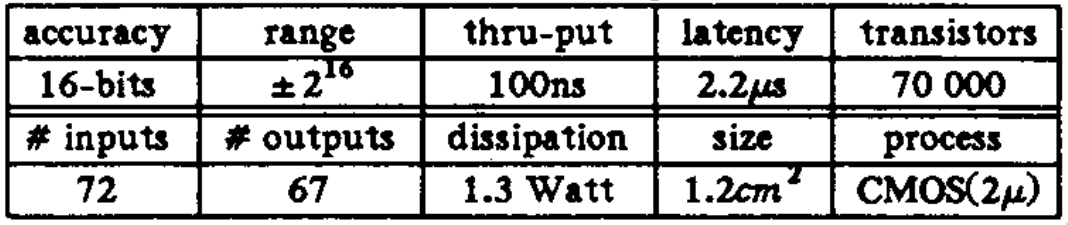
\includegraphics[width=0.75\textwidth]{archivos/CORDIC/1988_CORDIC_chip_features.png}
	\caption{Características de FP CORDIC}
	\label{graf:FP_CORDIC_features}
\end{figure}

Un diseño de CORDIC que mas se asemeja a las nuevas propuestas es el de \cite{de_lange_optimal_1988}, donde proponen un procesador de CORDIC de punto flotante y con \textit{pipelining} . Este chip podía realizar hasta $10^7$ rotaciones por segundo gracias al sistema de \textit{pipelining}. La entrada de valores era de 21 bits en punto flotante, 16 bits de mantisa y 5 bits para el exponente en complemento a dos. La salida era también en punto flotante (vea \ref{graf:Arq_FP_CORDIC}). Cabe destacar que el tipo usado en esta arquitectura no es estándar de IEEE.

\begin{figure}[ht]
	\centering
	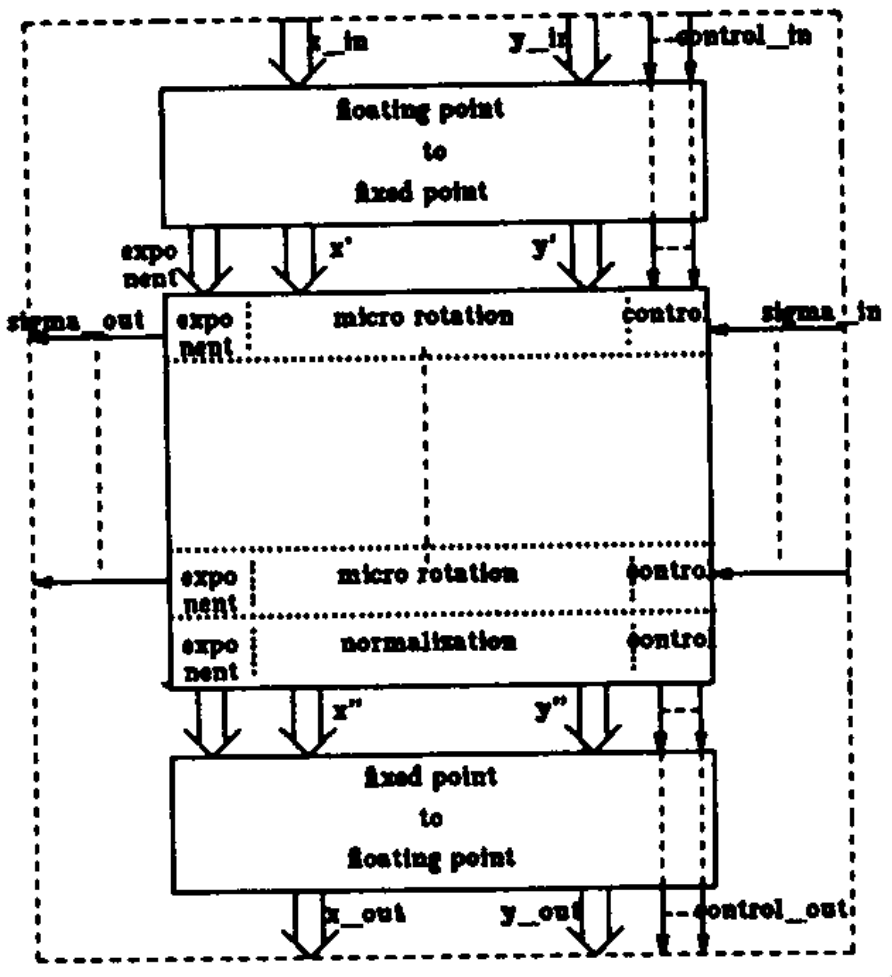
\includegraphics[width=0.5\textwidth]{archivos/CORDIC/1988_FP_CORDIC_Architecture.png}
	\caption{Arquitectura de FP CORDIC}
	\label{graf:Arq_FP_CORDIC}
\end{figure}

Para realizar las micro-rotaciones estipuladas anteriormente, la base del propio algoritmo, el procesador transforma el valor de punto flotante en punto fijo para el trabajo interno y posteriormente devuelve los valores en punto flotante. El valor $K$ es calculado en el momento de la conversión final del valor para devolver.

Como se puede observar, operar con punto fijo para realizar movimiento de bits es mucho mas fácil que tener que hacerlo directamente con punto flotante, por lo que los diseñadores generalmente, en muchos de los ejemplos mostrados posteriormente, realizan una conversión de punto fijo a punto flotante, o algunas veces directamente reciben valores en punto fijo para simplemente convertir una sola vez a punto flotante al final del algoritmo.

\cite{hekstra_floating_1993} presentaron un algoritmo de CORDIC de 32 bit de precisión con el estándar de IEEE 754. Este algoritmo puede realizar la rotación de un vector punto flotante $(x,y)$ con un ángulo de punto flotante $\alpha$. Este algoritmo fue diseñado con la intención de implementarlo en una unidad funcional para aplicaciones de procesamiento digital (DSP).

Para realizar las micro-rotaciones se da ciertos cambios, como el uso del método \textit{Block Floating Point} (BFP), el cual permite un uso de aritmética con punto fijo aunque el valor sea punto flotante. La ventaja de este método es la reducción de hardware y el coste de tiempo que puede traer las mismas funciones aritméticas comparadas a punto flotante pero sin perder el rango numérico que le da la ventaja a este.

\cite{zhou_double_2008} diseñaron un co-procesador FPGA basado en CORDIC con doble precisión (64 bits estándar IEEE 754) y \textit{pipelining}. Este diseño se centra explícitamente en las FPGAs, ya que como se puede ver anteriormente, y según lo descrito en este artículo, la mayoría se centraba dentro del área del ASIC, por lo que no había tantos ejemplos de implementaciones en hardware para FPGAs. Además, es de los pocos artículos con una implementación de 64 bits.

El diseño se basaba en tres fases: Transformación de los valores de punto flotante a punto fijo, método CORDIC y una fase de normalización, donde se devuelve el valor en punto flotante del IEEE 754.

Los resultados finales en este artículo muestran un \textit{speedup} considerable comparando a una CPU de la época, en concreto la AMD Athlon 64 Processor 3200+ (vea \ref{graf:2008_64FP_results_AMD}). Otros experimentos mostraban la reducción de espacio en el hardware comparados a otras soluciones y un error de resultados razonable.

\begin{figure}[ht]
	\centering
	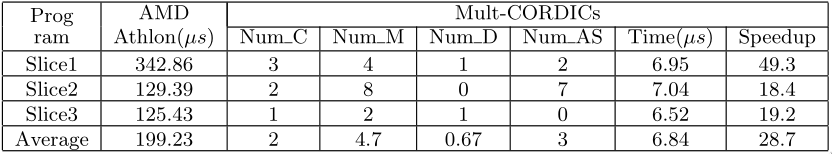
\includegraphics[width=\textwidth]{archivos/CORDIC/2008_64FP_results_AMD.png}
	\caption{Resultados de 64FP CORDIC y una CPU AMD Athlon 64 Processor 3200+. Num\_C es el número de co-procesadores de CORDIC usados en el experimento.}
	\label{graf:2008_64FP_results_AMD}
\end{figure}

\cite{nguyen_low-resource_2015} propone un CORDIC con punto flotante de baja latencia. El algoritmo propuesto reduce el número de iteraciones eligiendo un grupo particular de constantes para conseguir un resultado cercano al real.

La reducción del número de ángulos a escoger se basa en elegir los ángulos hasta llegar a un umbral particular para tener un error de cálculo muy cercano a como si se hiciera el de todas las constantes. Un punto a tener en cuenta es que el valor $K$ tendrá un valor diferente en cada operación del algoritmo, por lo que se tiene que recalcular en cada operación.

En cuanto a las entradas y salidas del algoritmo, la entrada es un valor del ángulo de punto fijo de 24 bits y las salidas son el $sin$/$cos$ con un valor de 32 bits IEEE 754 cada una.

\begin{figure}[ht]
	\centering
	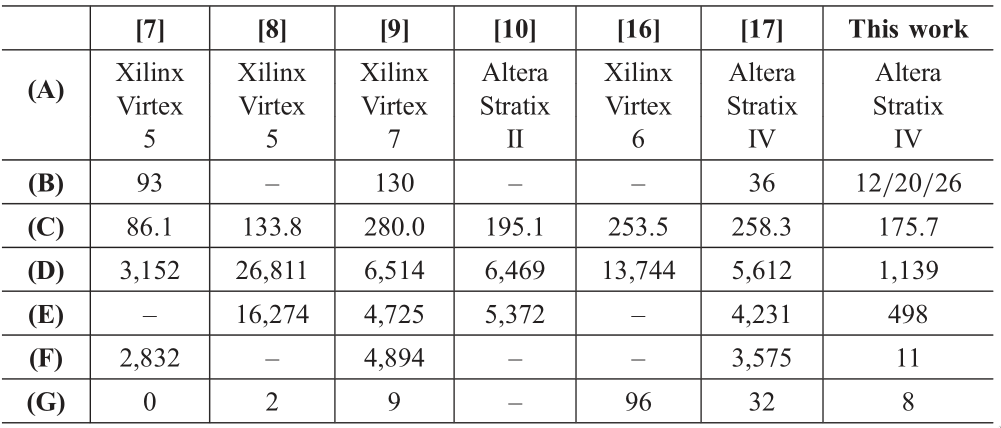
\includegraphics[width=0.7\textwidth]{archivos/CORDIC/2015_low-latency-fp.png}
	\caption{Tabla de comparaciones del CORDIC propuesto con otros trabajos parecidos. (A) Dispositivo. (B) Latencia (ciclos). (C) Frecuencia (MHz). (D) LUTs. (E) Registros. (F) Memoria. (G) DSP.}
	\label{graf:2015_low-latency-fp}
\end{figure}

Ahora se va a mostrar los artículos mas actualizados de CORDIC. Estos artículos muestran un interés general por el método y da confianza sobre el futuro de CORDIC.

\cite{hou_low_2019} diseñan un algoritmo CORDIC usando el estándar IEEE 754 de doble precisión (64 bits).

La metodología del tratamiento de los datos es muy parecida a la literatura descrita anteriormente, la entrada es un valor de punto flotante que en un módulo de pre-procesamiento realiza una conversión a punto fijo y además se procesa las excepciones que podrían aparecer en este momento, como por ejemplo un $NaN$.

La unidad de procesamiento de CORDIC utiliza el llamado \textit{Point 4-step Iterative Processing Unit}, el cual ocupa mas espacio que un CORDIC tradicional, pero logra calcular por cada ciclo 16 micro-rotaciones de CORDIC, reduciendo efectivamente el tiempo por 4 (vea \ref{graf:2019_4-step-64bit}).

\begin{figure}[ht]
	\centering
	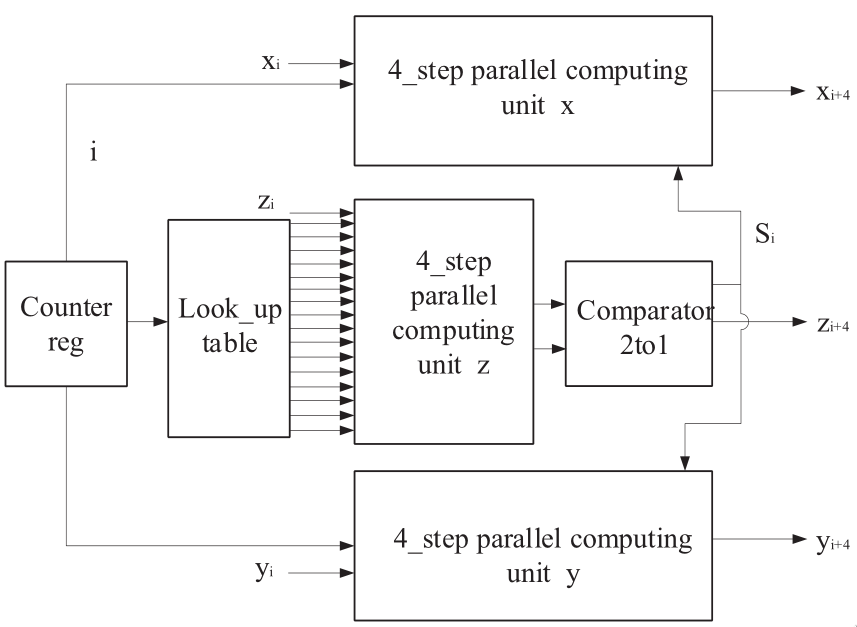
\includegraphics[width=0.75\textwidth]{archivos/CORDIC/2019_4-step-64bit.png}
	\caption{Unidad de procesamiento de CORDIC de doble precisión}
	\label{graf:2019_4-step-64bit}
\end{figure}



















